\documentclass[11pt,a4paper]{scrreprt}

\usepackage[utf8]{inputenc}
\usepackage[italian]{babel}

\usepackage{amsmath}
\usepackage{graphicx}
\usepackage{tabularx}

\usepackage{parskip}

\usepackage{placeins}

\usepackage{url}
\usepackage{fancyvrb}
\usepackage{fancyref}
\usepackage[hidelinks]{hyperref}

\author{L. De Sano, A. Donizetti}
\title{\textsc{FIC}: Fractal Image Compression}
\date{Luglio 2015}

\begin{document}
\maketitle

\tableofcontents

\chapter{Introduzione}

La compressione di immagini tramite frattale è una tecnica di compressione \textit{lossy}, quindi con perdita di qualità. Questa metodo di compressione è adatto soprattutto per comprimere texture o immagini della natura, a seguito del fatto che in queste immagini spesso delle parti assomigliano molto a delle altre; la compressione tramite frattali permette di memorizzare queste parti e di utilizzare poi per ricreare l'immagine originale. La compressione tramite frattali, a differenza dei metodi di compressione basati sui pixel come \textit{JPEG}, \textit{GIF} o \textit{MPEG}, non memorizza nessuna parte dell'immagine, ma solo le informazioni sulla sua ricostruzione vengono immagazzinate. Una volta che un'immagine è stata processata può essere ricostruita alla dimensione preferita, senza quella perdita di qualità che si verifica con le normali tecniche di compressione.

In questo documento daremo una breve descrizione del problema, esplorandone i principali aspetti teorici e forniremo un'implementazione di un algoritmo di compressione in linguaggio \texttt{MATLAB} che, per quanto semplice, permette di ottenere dei risultati soddisfacenti.

\chapter{Aspetti teorici}

\section{Introduzione ai frattali}

Un frattale è un oggetto geometrico che si ripete nella sua forma, allo stesso modo, su diverse scale. Questo comportamento fa si che ingrandendo una sua qualsiasi componente si ottiene comunque una figura simile all'originale. In linea di massima possiamo dire che se si considera l'insieme $F$ un frattale, $F$ dovrebbe avere le seguenti proprietà:

\begin{itemize}
\item $F$ ha dettagli ad ogni scala d'ingrandimento;
\item $F$ gode di autosimilitudine (a qualunque scala si osservi, presenta sempre gli stessi caratteri globali);
\item la dimensione frattale di $F$ è maggiore della sua dimensione topologica;
\item esiste un algoritmo relativamente semplice per costruire $F$.
\end{itemize}

% dobbiamo definire dimensione frattale e dimensine topologica? qui c'è qual che serve http://www.vanderbilt.edu/AnS/psychology/cogsci/chaos/workshop/Fractals.html

% mettere qualche esempio di frattale di base con la costruzione iterata?

Un esempio di oggetto geometrico secondo i principi di costruzione di un frattale e che rispetta le proprietà elencate è la curva di \textit{Koch}. La costruzione comincia con una linea di lunghezza $1$ chiamata \textit{initiatior}. Da questa linea si rimuove il terzo centrale e lo si sostituisce con due linee della stessa lunghezza della parte rimossa. Questa nuova forma viene chiamata \textit{generator}. La prima parte della costruzione è mostrata in figura \ref{fig:k1}.

\begin{figure}[!ht]
\centering
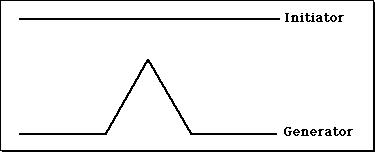
\includegraphics[scale=0.55]{images/koch1.png}
\caption{Initiator e generator per la curca di Koch}
\label{fig:k1}
\end{figure}

La regola può essere nuovamente applicata su ogni linea, così da andare a sostituirla ogni volta come fanno nel passaggio da \textit{initiator} a \textit{generator}. Il secondo livello è visibile in figura \ref{fig:k2}.

\begin{figure}[!ht]
\centering
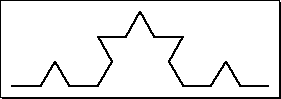
\includegraphics[scale=0.55]{images/koch2.png}
\caption{Livello 2 per la curca di Koch}
\label{fig:k2}
\end{figure}

\FloatBarrier

Una volta che la procedura è avviata può proseguire a piacimento. Il terzo e il quarto livello sono visibili nelle figure \ref{fig:k3} e \ref{fig:k4} rispettivamente.

\begin{figure}[!ht]
\centering
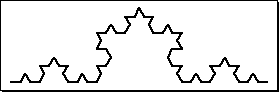
\includegraphics[scale=0.55]{images/koch3.png}
\caption{Livello 3 per la curca di Koch}
\label{fig:k3}
\end{figure}

\begin{figure}[!ht]
\centering
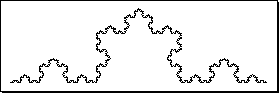
\includegraphics[scale=0.55]{images/koch4.png}
\caption{Livello 4 per la curca di Koch}
\label{fig:k4}
\end{figure}



\section{Iterated Function System}







\end{document}
